\documentclass[12pt]{article}
\usepackage{geometry}
\geometry{verbose, letterpaper, tmargin = 2.54cm, bmargin = 2.54cm,
  lmargin = 2.54cm, rmargin = 2.54cm}
\geometry{letterpaper}
\usepackage{graphicx}
\usepackage{amssymb}
\usepackage{amsmath}
\usepackage{amsfonts}
\usepackage{setspace}
\usepackage{booktabs}
\usepackage{ragged2e}
\usepackage{verbatim}
%\usepackage[sectionbib]{chapterbib}
\usepackage{amsmath}
\usepackage{longtable}
\usepackage{multirow}
\usepackage{array}
\usepackage{tabu} % for spacing between rows in longtable
\usepackage{titlesec}
\usepackage{url}

\usepackage{lineno}
\usepackage{xcolor}
\renewcommand\linenumberfont{\normalfont\tiny\sffamily\color{gray}}
\modulolinenumbers[2]

\widowpenalty=10000
\clubpenalty=10000

% Linux Libertine:
\usepackage{textcomp}
\usepackage[sb]{libertine}
\usepackage[varqu,varl]{inconsolata}% sans serif typewriter
\usepackage[libertine,bigdelims,vvarbb]{newtxmath} % bb from STIX
\usepackage[cal=boondoxo]{mathalfa} % mathcal
\useosf % osf for text, not math
\usepackage[supstfm=libertinesups,%
  supscaled=1.2,%
  raised=-.13em]{superiors}

\textheight 22.0cm

\usepackage[round]{natbib}
\bibpunct{(}{)}{;}{a}{}{}

%%%%%%%%%%%%%%%%%
\hyphenation{meta-pop-ulation meta-pop-ulations sub-pop-ulations
  sub-pop-ulation e-con-o-mist en-vi-ron-men-tal pri-or-i-ti-za-tion}

\title{TODO New title needed: Ecological portfolio theory:
  When should conservation biologists play investment banker?}

\author{Sean C. Anderson$^{1\ast}$,
  Andrew B. Cooper$^2$,
  and Nicholas K. Dulvy$^1$}
\date{}

\usepackage{lineno}
\usepackage{xcolor}
\renewcommand\linenumberfont{\normalfont\tiny\sffamily\color{gray}}

% remove numbers in front of sections:
\makeatletter
\renewcommand\@seccntformat[1]{}
\makeatother

\begin{document}

%\maketitle
% \noindent
% $^1$Earth to Ocean Research Group,
% Department of Biological Sciences,
% Simon Fraser University,
% Burnaby, British Columbia, Canada
%
% \noindent
% $^2$School of Resource and Environmental Management,
% Simon Fraser University,
% Burnaby, British Columbia, Canada
%
% \noindent
% $^{\ast}$Corresponding author:
% Earth to Ocean Research Group,
% Department of Biological Sciences,
% Simon Fraser University,
% Burnaby, British Columbia, Canada,
% Email: sean\_anderson@sfu.ca

%\noindent
%Running head: Conserving Ecological Portfolios

%\noindent
%Keywords:
%biocomplexity,
%diversity-stability,
%Modern Portfolio Theory,
%portfolio effect,
%response diversity,
%risk,
%spatial heterogeneity,
%synchrony
% ($\le$ 8)

\clearpage
\linenumbers
\begin{spacing}{1.25}
\input{ms}
\bibliographystyle{apalike}
\bibliography{/Users/seananderson/Dropbox/tex/jshort,/Users/seananderson/Dropbox/tex/ref3}
\clearpage
\LTcapwidth=\textwidth
\bibpunct{}{}{;}{a}{}{;}
\singlespacing
\begin{small}
\begin{longtable}{>{\RaggedRight}p{3.6cm}>{\RaggedRight}p{7.3cm}>{\RaggedRight}p{3.6cm}}

\caption{Selected ecological theory relevant to ecological portfolios.}\\

\toprule

\textbf{Ecological theory} &
\textbf{Relevance to ecological portfolios} &
\textbf{Selected references} \\

\midrule
\multicolumn{2}{l}{\textbf{Sources of portfolio structure}} \\
\midrule

Theory of island biogeography &
Explains a source of diversification for ``islands'', which have a portfolio-like structure. Larger islands may have higher levels of portfolio diversification. &
\citep{macarthur1967}\\

Metapopulations &
Subpopulations can act as diverse ecological assets as part of a metapopulation portfolio. Metapopulations usually have exchange between subpopulations (ecological assets), which may not have an analogy in financial portfolios. &
\citep{levins1969}\\

Functional groups &
Species that perform separate ecological functions can form ecological assets as part of an ecological portfolio. &
\citep{walker1992, thibaut2012}\\

Community ecology &
We can represent species as assets and a community of species as a portfolio. Species interactions such as predation and competition may complicate the analogy. &
\citep{morin2011}\\

\midrule
\multicolumn{2}{l}{\textbf{Causes of diversification and portfolio dynamics}}\\
\midrule


Spatial heterogeneity &
Heterogeneity in habitat may create pockets of diverse ecological assets. &
\citep{oliver2010,parn2012}\\

Moran effect &
Identifies that similar environments will induce similar population responses decreasing the diversity of a portfolio. Ecological assets that are further apart are expected to provide greater diversification. &
\citep{moran1949, ranta1998}\\

Biocomplexity &
Identifies that subpopulations can display a range of biological traits and behaviours and that these ranges can form portfolio diversification &
\citep{hilborn2003, hutchinson2008}\\

Synchrony &
Often loosely used to referred to correlation between ecological assets. Defined quantitatively by \citet{loreau2008} as a diversity-independent metric of correlation. The benefit of diversification is greater when synchrony of ecological assets is low. &
\citep{ranta1998, loreau2008, moore2010}\\

Response diversity &
Identifies elements of ecological systems that cause them to respond differently to perturbation. Potentially the most important aspect of ensuring stable portfolios as the magnitude and frequency of environmental stressors (e.g.\ climate change) increase. &
\citep{elmqvist2003, loreau2008, loreau2013}\\

Intraspecific trait variation &
Identifies that variation among individuals in a population can form an important component of diversity and affect population dynamics. Individuals could be thought of as ecological assets. &
\citep{bolnick2011}\\

Unified neutral theory of biodiversity and biogeography &
Asks what community dynamics we would observe if species were functionally equivalent. We can think of a neutral community with ecological equivalence as an un-diversified portfolio compared to a diversified portfolio in which species show functional diversity. &
\citep{hubbell2001}\\

%Compensatory dynamics and complementarity & … & [65]\\

%Competitive interactions & … & [37]\\

\midrule
\multicolumn{2}{l}{\textbf{Risk-reduction consequences of diversity}}\\
\midrule

Diversity-stability hypothesis &
Identifies when and why certain types of diversity correspond with certain types of stability. Another name for many of the same concepts that ecological portfolio theory addresses.  &
\citep{ives2007, loreau2013}\\

Statistical averaging &
Some level of reduction in variability in a portfolio is inevitable due to averaging of asset time series &
\citep{doak1998}\\

Portfolio effect &
A term to represent the benefit of a system existing as a portfolio of ecological assets instead of a single homogeneous asset &
\citep{schindler2010, thibaut2013}\\

Insurance hypothesis &
Similar to the portfolio effect, but emphasizes that negative covariance reduces the likelihood that all assets will decline at the same time. &
\citep{yachi1999,valone2008}\\

\bottomrule
\label{tab:theory}
\end{longtable}
\end{small}

\clearpage
\LTcapwidth=\textwidth
\bibpunct{}{}{;}{a}{}{;}
\singlespacing
\begin{footnotesize}

\begin{longtable}{>{\RaggedRight}p{2.7cm}>{\RaggedRight}p{3.3cm}>{\RaggedRight}p{3.9cm}>{\RaggedRight}p{4.2cm}}

\caption{Attributes of financial and ecological data and their implications for ecological portfolios}\\
\toprule

\textbf{Data attributes} &
\textbf{Financial portfolios} &
\textbf{Ecological portfolios} &
\textbf{What this means for ecological portfolios}\\

\midrule

Interdependence &
A diverse portfolio is unlikely to have strong dependence between assets &
Populations may be strongly impacted by changes in other populations of the same species (e.g.\ competition or migration) or other species (e.g.\ predation) &
Interactions needs to be accounted for; forecasts may be less reliable\\

Measurement error &
Reported asset value is the true value that impacts an investor &
Recorded data typically includes substantial measurement error and may be biased &
Uncertainty needs to be propagated through analyses\\

Frequency and duration &
High frequency (e.g.\ seconds), regular recording intervals, missing values rare, long durations &
Lower frequency (often years), sometimes irregular recording intervals, missing values common, often short durations &
Greater uncertainty in optimal solutions; time-series methods require unique approach (e.g.\ missing values may need to be imputed, autocorrelation different)\\

Synchrony &
Relatively low synchrony for diversified portfolios &
Relatively high synchrony for similar populations or species; potential asynchrony due to species interactions &
Potentially less benefit from portfolio diversification; species interactions may alter portfolio dynamics\\

Mean-variance scaling &
Variance scales directly with investment &
Variance may scale indirectly with investment if asset size itself is considered an investment weight (Fig.~\ref{fig:salmonport}) &
The mean-variance relationship may need to be accounted for\\

Number of assets &
Typically unlimited; generally high &
Typically limited; generally low &
Potentially less opportunity for portfolio diversification\\

\bottomrule
\label{tab:data}
\end{longtable}
\end{footnotesize}

\begin{figure}[htbp]
\centering 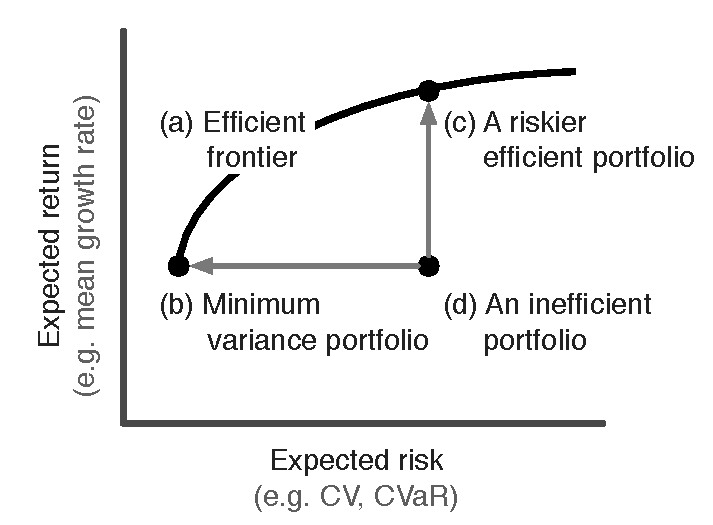
\includegraphics[width=3.5in]{efficient-frontier-fig.pdf}
\caption{An introduction to Modern Portfolio Theory mean-variance optimization.
  In finance, portfolios are formed by choosing how much to invest in various
  assets. Modern Portfolio Theory focuses on identifying the set of portfolios
  that optimizes the trade-off between expected return (`mean') and expected
  risk (`variance'). \textbf{(a)} This set of portfolios is referred to as the
  efficient frontier. A manager would choose a portfolio on the efficient
  frontier, but the relative position would depend on risk tolerance.
  \textbf{(b)} The minimum variance portfolio achieves the lowest expected
  risk; the remaining risk is said to be undiversifiable. \textbf{(c)} A
  risker, but still efficient portfolio. \textbf{(d)} An example inefficient
  portfolio, which has a lower expected return than (c) and greater expected
  risk than (b). Adapted from \citet{hoekstra2012}.} \label{fig:mpt}
\end{figure}

\clearpage

\begin{figure}[htbp]
\centering 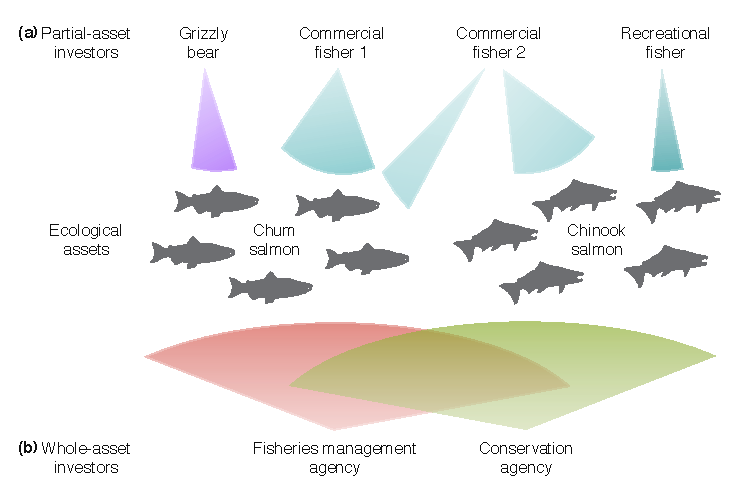
\includegraphics[width=5in]{salmon-portfolios.pdf} \caption{There
  are multiple ways of investing in ecological portfolios. In this example,
  investors are shown along the top and bottom and ecological assets are shown
  in the middle (populations of chum salmon, \textit{Oncorhynchus keta}, and
  Chinook salmon, \textit{Oncorhynchus tshawytscha}). The shaded arcs indicate
  investment. \textbf{(a)} Partial-asset investors invest by removing portions
  of the salmon populations --- the salmon that commercial fisher 1 removes are
  unavailable for the grizzly bear. These investors can often change their
  investment with ease. For example, commercial fisher 2 could decide to fish
  more Chinook and less chum salmon. Most financial portfolio theory is
  developed around this paradigm. \textbf{(b)} Whole-asset investors invest in
  entire populations. These investors can share assets but may have different
  goals for their portfolio. They can adjust their investment by managing
  properties of the population itself. For example, the fisheries management
  agency could reduce fishing of chum salmon to allow the population to grow.
  The conservation agency could fund habitat restoration for Chinook salmon to
  increase carrying capacity and expand their investment.}
\label{fig:salmonport}
\end{figure}

\begin{figure}[htbp]
\centering
%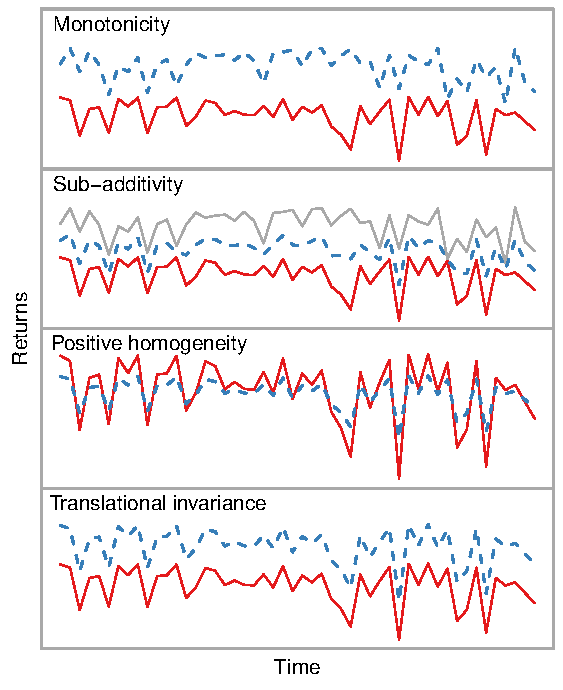
\includegraphics[width=2.6in]{coherence-axioms.pdf}
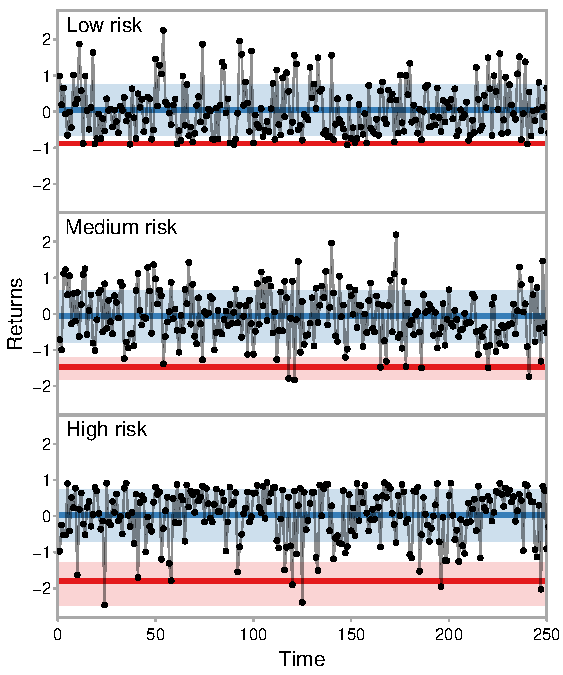
\includegraphics[height=3.10in]{skewness-abundance.pdf}
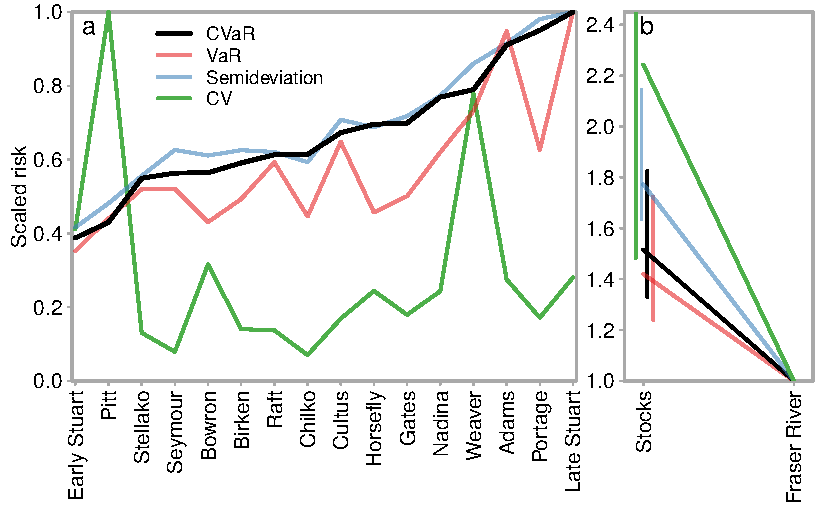
\includegraphics[height=2.11in]{compare-risk-and-portfolio-scale.pdf} \caption{
  Symmetric vs.\ downside risk measures. \textbf{(Left panel)} An illustration
  of three systems with the same symmetric variability but different levels of
  downside risk. The y-axis denotes rate of change of abundance or biomass
  (``returns'' in financial terminology). The dark blue line represents the
  mean and the blue shaded region represents $\pm$ one standard deviation --- a
  measure that does not account for the asymmetric property of risk. The red
  line represents the 95\% CVaR (conditional value at risk) and the red shaded
  region represents the region below the 95\% VaR (value at risk). CVaR and VaR
  are both downside risk measures that accurately identify higher risk systems.
  \textbf{(Right panel)} \textbf{(a)} Symmetric and downside risk metrics
  applied to annual returns of sockeye salmon stocks in the Fraser River (data
  from \citeauthor{dorner2008} \citeyear{dorner2008}). Stocks are ordered by
  increasing CVaR. Symmetric (CV) and asymmetric (all other) risk metrics
  differ considerably in their rank order of risk for the different stocks.
  \textbf{(b)} The portfolio effect calculated for the same salmon stocks using
  the four risk metrics. Sloped lines at the stock level represent the mean
  portfolio effect (how many times more variable or risky the average stock is
  than the Fraser River as a whole) and the vertical segments show the
  interquartile range.} \label{fig:risk}
\end{figure}

\end{spacing}
\end{document}
